\chapter{TCP server and Serialization}
\minitoc

In this chapter we talk about the TCP protocol. in section \ref{tcp_lab} we describe the assignment. In section \ref{tcp_solution} we describe our solution. in section \ref{tcp_example} we provide an example run of the solution. In section \ref{tcp_reflection} we try to connect the example to the theory behind. 

\section{lab description}
\label{tcp_lab}
\textit{The purpose of this week’s lab exercise is to develop a simplified version of web server for task manager that runs on TCP protocol.}\\

\textit{The task manager TCP server and its clients follow a strictly predefined structured communication based on the following conversational protocol.}

\begin{itemize}
\item \textit{Initially a client will send a command to the server indicating that it wishes to consume the particular service offered by the server through the mentioned command.}\\

\item \textit{After receiving a command from the client, the server will respond by sending the same command back to the client indicating it’s readiness to provide the service mentioned in the command.}\\

\item \textit{Soon after receiving the command from the server, the client will send necessary data to the server to further process the command on the server side. In case of POST and PUT commands, the client will send a Task object, where as in case of GET or DELETE commands, the client will send an attendant’s name or a task id respectively.}\\

\item \textit{Finally, after processing the command the server will send back the results to the client. In case of GET command, the server will return a list of tasks object (List\textless Task \textgreater) to the client. On the other hand, it will simply return the result of that command (e.g. task deleted). The result could also contain an error message if any (e.g. task Id not found in the task list).}
\end{itemize}


\textit{In this lab exercise, you are required to develop the code for the following functionality.}\\

\begin{itemize}
\item \textit{Develop java serialization classes for task-manager-xml using Java Architecture for XML Binding (JAXB) APIs (by annotating java classes) to handle deserialization/serialization from/to task-manager-xml in the server.}\\

\item \textit{Develop TaskManagerTCPServer and TaskManagerTCPClient classes to implement the above described functionality of server and client that communicate on the TCP protocol.}\\

\item \textit{[Optional] The server described above can only handle one single client at a time in each run. In order to make the server more robust and handle multiple clients concurrently, one may follow the approach suggested in the page. 173 of the course textbook [DS], to create a new connection for every client request that will run on a separate thread. Therefore, develop a TaskManagerTCPServer that can handle multiple concurrent clients.}\\

\item \textit{[Optional] The functionality of TaskManagerTCPServer can be extended to offer more commands (e.g. OPTIONS, HEAD) similar to the HTTP protocol. In case of OPTIONS command, one may describe the list of commands offered by the server, where as for HEAD, one may only provide the number of tasks available for a given attendant instead of sending all the available tasks to the client.}\\

\end{itemize}

\section{Solution}
\label{tcp_solution}

Due to the general pressure of the study we did not find the time to elaborate much on this excersize. Hence the optional parts are not implemented.\\

We use JAXB API to provide persistence for the taskmanager objects. JAXB is java middleware capable of marshalling and unmarshalling java objects into xml and back into java objects, in this case a 'taskmanager' object with a related collection of ‘Task’ objects. To send the taskmanager object over TCP/IP, objects are transformed into bytes by ObjectInputStream and ObjectOutputStream (only objects that are serializable may be written as a bytestream).   \\ 

Our TCP server first opens a serversocket on a specified port and continues to listens for clients . A client instantiates a socket specifying the serversocket's address and port number. The client and server then communicates by passing byte streams through the agreed upon port. The transmission of bytes is done with ObjectInputStream and ObjectOutputStream methods.  \\

\subsubsection{Serialization}
Information in OO programs are typically stored as data structures whereas data in the messages used to communicate in distributed systems are binary. So, no matter the communication protocols used the data structures need to be flattened before transmitting and then reassembled at the other end.



\subsubsection{Byte Stream}
ObjectInputStream/ObjectOutputStream are java methods for transforming serializable java objects to and from bytestreams. \\ 

In Java,  serializable objects can be sent through a connection by  ObjectInputStream and ObjectOutputStream classes which transforms an object or a graph of objects into an array of bytes (for storage or transmission), and back into objects again. \\

Our server and client communicates by passing bytes in and out of matching inputstreams and outputstreams. Command messages (requests) are passed via the writeUTF and received by the readUTF methods as DataStreams. The Task and taskmanager objects, implementing serializable, are sent via ObjectOutputStream and received by ObjectInputStream. \\

The server responds to requests by sending the request back. The client waits for this confirmation before proceeding. \\

\subsubsection{JAXB}
Serialization and deserialization to and from xml is done with the JAXB API. Quoting Oracle; \textit{JAXB provides methods for unmarshalling (reading) XML instance documents into Java content trees, and then marshalling (writing) Java content trees back into XML instance documents.} \\

JAXB uses annotations to achieve this. We annotate the Task and Taskmanager Java objects and JAXB then knows how to convert these annotated objects into an xml tree-structure and back into an object graph.\\

\begin{lstlisting}
@XmlRootElement(name = "taskmanager") // JAXB annotation
public class TaskManager implements Serializable{

	@XmlElementWrapper(name = "tasks") // 
    @XmlElement(name = "task")
    public List<Task> tasks;
}
\end{lstlisting}

\subsubsection{TCP}

The Transmission Control Protocol (TCP) is one of the main protocols of the transport layer of the TCP/IP suite. TCP provides reliable and ordered streams over the internet. TCP is located at the transport layer where it  receives data from the application layer and sends data to the lower level internet layer IP protocol. \\

TCP transforms data into packets, a sequence of bytes consisting of a headder (metadata) and a body (the data). \\

The TCP server in our solution first connects to a serversocket and then waits for incoming requests on the port bound to the socket. Note this is a blocking call and the server will wait for a client to connect. The Client creates a socket on the same port which takes the server's InetAddress and the port it is listening on as arguments. \\

\section{example run}
\label{tcp_example}

In our example the server sends out confirmation messages to the client for each request received. The client proceeds, only after receiving an acknowledgement of its request. This mimics the way the TCP protocol uses acknowledgements (acks) to confirm packet reception. Acks are the way the TCP protocol achieves \textit{reliability}. A client will wait for an ack and if none arrives it retransmits the package.\\   

After establishing a socket connection between client and server the client sends a request to the server. The server responds by sending an ack to the client (in this case the ack is the request itself).
% \lstinputlisting{TCPserver.java}

\begin{lstlisting}[caption= server sends an ack to a request]
while(running){
         // client request
         String message = dis.readUTF(); // [blocking call]
         // accept client request by returning the (request) message
         dos.writeUTF(message);    

\end{lstlisting}

The client continues, only after receiving the ack from the server.
\begin{lstlisting}[caption=client request and wait for ack]
String message = "POST";
dos.writeUTF(message);		// send the request
response = dis.readUTF();	// wait for ack [Blocking call ]

Task t = new Task();
t.name = "Tout les circles";
t.id = "one more cup of coffe";
t.date = "15-09-2013";	
t.description = "recondre";
t.status = "mais jai le plus grande maillot du monde";
t.attendants = "bjarne, lise, hans, jimmy";

// if server acknowledges
if(response.equals(message)){
   	ous.writeObject(t);
}else{
   	System.out.println("Client: the server did not acknowledge the request.");
}
\end{lstlisting}


The client-server uses readUTF() and writeUTF() to send requests and acks but in order to send an object they use writeObject() and readObject() to transform the object into a byte stream to send over the socket. \textit{Only objects implementing serializable can be transmitted by writeObject().} After receiving the bytestream we cast it back into an object.\\

After executing a POST operation the server then proceeds to persist the taskmanager object by marshalling it with JAXB.

\begin{lstlisting}[caption=server POST]
// expect an object from the client
if(message.equals("POST")){   
	Task t = (Task) ois.readObject(); // 
	serializer.allTasks.tasks.add(t);
    serializer.Serialize();	
}
\end{lstlisting}

Before the example run the taskmanager xml document looked like this:

\begin{lstlisting}[caption=xml before run]
<?xml version="1.0" encoding="UTF-8" standalone="yes"?>
<taskmanager>
	<tasks>
		
		<task id="handin-01" name="Submit assignment-01" date="16-12-2013"
			status="not-executed">
			<description>
				Work on mandatory assignment.
			</description>
			<attendants>student-01, student-02</attendants>
		</task>	
	</tasks>
</taskmanager>

\end{lstlisting}


After the run, in which the client requested the server's POST method with a new Task, the xml document looks like this:

\begin{lstlisting}[caption=xml after POST]
<?xml version="1.0" encoding="UTF-8" standalone="yes"?>
<taskmanager>
	<tasks>
		<task id="handin-01" name="Submit assignment-01" date="16-12-2013" status="not-executed">
			<description>
				Work on mandatory assignment.
			</description>
			<attendants>student-01, student-02</attendants>
		</task>
		<task id="one more cup of coffe" name="Tout les circles" date="15-09-2013" 
		status="mais jai le plus grande maillot du monde">
			<description>recondre</description>
			<attendants>bjarne, lise, hans, jimmy</attendants>
		</task>
	</tasks>
</taskmanager>
\end{lstlisting}

Not included in this summary, but in the complete example the client also requests the GET method and the PUT method wanting to change the new task's description property. Finally, the client requests the DELETE method with the taskid 'handin'01' parameter. After the run the xml document now looks like this:

\begin{lstlisting}[caption=xml after PUT]
<?xml version="1.0" encoding="UTF-8" standalone="yes"?>
<taskmanager>
	<tasks>
		<task id="one more cup of coffe" name="Tout les circles" date="15-09-2013" status="mais jai le plus grande maillot du monde">
			<description>recondre les roix</description>
			<attendants>bjarne, lise, hans, jimmy</attendants>
		</task>
	</tasks>
</taskmanager>
\end{lstlisting}



















\begin{figure}[H]
\centering
\caption{console output tcp client}
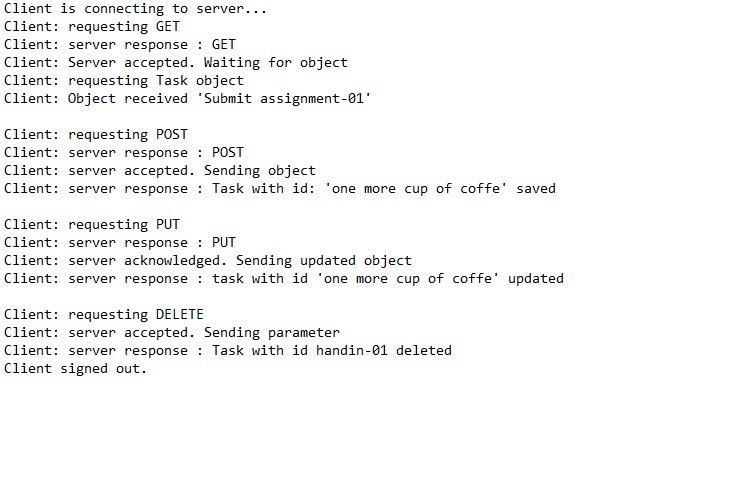
\includegraphics[scale=0.7]{images/TCP_run_client.png}
\end{figure}
\vspace{10pt}


\begin{figure}[H]
\centering
\caption{console output server}
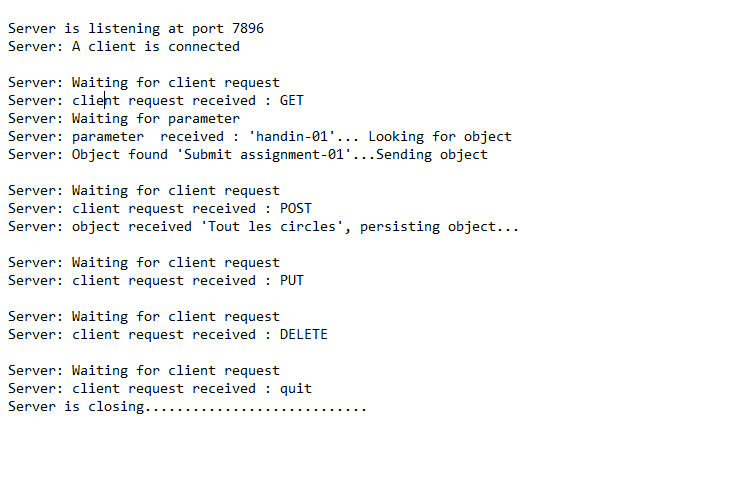
\includegraphics[scale=0.7]{images/TCP_run_server.png}
\end{figure}
\vspace{10pt}

\section{Reflection}
\label{tcp_reflection}

We have used this example to demonstrate and experiment with the TCP/IP suite. There are two transport protocols in the TCP/IP suite; UDP and TCP. UDP transfers text messages and TCP transfers byte streams. Unlike UDP, TCP is reliable and ordered. TCP can provide guarantees as to the ordering of its messages i.e., messages arrive in the order they were sent. It does so by giving every packet a number and then ordering the packets on arrival. TCP provides guarantees as to the delivery of the messages i.e, the message eventually arrive. It does so by using acknowledgements and retries (resend messages).   \\

In contrast, the underlying network protocol (the IP protocol ) offers only 'best-effort' semantics, there is no guarantee of delivery and packets can be lost, duplicated, delayed or delivered out of order. IP delegates the task of providing a reliable service to other layers, namely the TCP layer atop it. This nicely demonstrates the end-to-end principle. Application specific functionality should reside at the end hosts.\\



Network layers send IP packets to (IP)addresses accross the network. The transport layer's UDP and TCP protocols sends IP packets to processes instead of addresses. TCP provides guarantees about reliability, ordering etc which UDP does not and this makes TCP well suited for server-client architectures in distributed systems. \\

Our simple example mimiced the way the TCP protocol achieves reliability. By sending acknowledgements our client-server is, in principle, capable of achieving reliability. It could be made to resend a packet in case of no response from the other end. Off course things like latenzy, troughput or duplicate packages come into play here. \\

The code in our solution is very much a 'proof-of-concept'. The code style could only have been done better but since this was a course in Distributed Systems, and not in code writing norms, we chose to leave the code as is and concentrate on the theory behind.  \\

As with many other examples, we did not have time to implement the optional parts of the assignment. This is much regrettable but we feel we at least have had a good introduction to the TCP/IP suite.

